% % % % % % % % % % % % % % % % % % % % %
% 	         BACKGROUND
% % % % % % % % % % % % % % % % % % % % %
\section{Background}
\label{awa:background}
% Perhaps you want to cite the seminal paper of \citet{Turing1937}, or
% prior~\cite{Goedel1931} and concurrent~\cite{Church1936} work.
\todo{SIGNPOSTING TEXT!!}

\subsection{The Game of Minesweeper} \label{awa:minesweeperGameContext}

Minesweeper is a popular logic game which was first released in 1989 as part of Microsoft Windows. It is a grid-based logic game, where the player is presented with a finite board featuring covered cells that may contain either a mine or an empty space. The player is tasked with uncovering all empty spaces on the board, usually done by deducing non-empty cells via the numbers inscribed on each cell stating the number of mines in the surrounding 8 cells.
In addition to the basic logic, the standard game also allows the player to keep track of mines by flagging suspected cells with mines, allows the player to execute a "chord" (explained bellow), and further helps them by automatically uncovering neighbours of a cell inscribed with 0. In the original game, the standard difficulties are comprised of Beginner (shown in \cref{fig:beginnerExample}), Intermediate, and Expert. These difficulties correspond to boards of 9 by 9 with 10 mines, 16 by 16 with 40 mines, and 30 by 16 with 99 mines (respectively).

\textit{chording} is a create-comfort feature which can be triggered on any revealed cell with a hint from one to eight, as long as the number of flags placed on the neighbouring cells (both immediate and diagonal) are equal to the hint number inscribed on the cell. The action itself will then open all neighbouring cells which are covered and un-flagged.

This feature is most used to save time and clicks when all cells are found in a 3x3 area, and is typically counted as the actual amount of mouse button clicks, meaning that there are less clicks actually counted compared to manually opening the neighbouring, known safe, cells.

\begin{figure}[htbp]
    \centering
    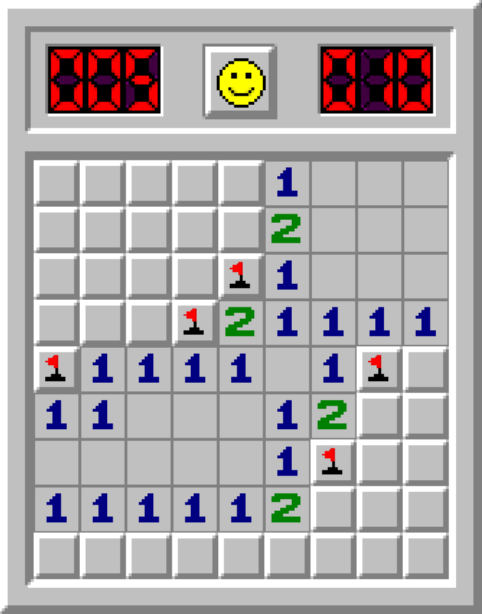
\includegraphics[width=0.5\linewidth]{embeddables/9x9ExampleBoardV2.png}
    \caption{A partially completed beginner board showing covered cells, covered cells flagged by the user, and opened cells with hints 0-8 indicating the number of neighbouring (both immediate and diagonal) mines.}
    \label{fig:beginnerExample}
\end{figure}

\subsection{Minesweeper Difficulty Metrics, their Purpose, and Flaws} \label{awa:minesweeperImprovementDrive}
% \subsubsection{Drive for improvement} \hfill \\
As with all games, particularly dedicated players aim to incrementally improve their skill, subject to some metric indicative of their performance. In minesweeper, there are two main metrics used in this process. The primary metric is solve time. For a player, solve time primarily serves as an objective reward which indicates how skilful the player was, and lets them adjust their methods accordingly over multiple plays to optimise their performance.

Solve time is not influenced just by player ability, but also by field difficulty.
When evaluating their play with the aim to improve, the player needs to "normalise" the performance they were expecting to display, to adjust for the field's difficulty.
\
This is why players typically try to improve over randomised placements of a fixed number of mines within a field of a fixed size, since it reduces difficulty variance, however games generated subject to these conditions still do not necessarily have the same difficulty over different randomisations, as different configurations can produce sequences of mines that might force more guesses, require moves of varying difficulty, bias speed of travel around the grid, capacity to memorise mines, pattern recognition, \textit{etc} (these ideas will be explained more concretely in \cref{sec:evaluation}).

In an effort to further mitigate this, \citet{3BVmetric} created the "3BV" score, a metric which simply counts the minimum number of necessary clicks to solve a board without using any flags. This is calculated upon completion of the board, and is used retrospectively by the player to adjust their belief on the quality of their performance.
% \todo{write an argument on scores being used retrospectively.}
\
This is still non-exhaustive, as is acknowledged by the creator of the aforementioned 3BV, who presents as an example two fields they had solved themselves in the same time (20s) with widely differing 3BV scores (38 and 72) shown below in \cref{fig:3BVbad}.
The general sentiment in the wider competitive Minesweeper community is similarly critical of its usefulness as a difficulty indicator on its own, as can be seen in some of the many online forum discussions on the topic\cite{redditComment1, redditComment2, redditComment3}.

\begin{figure}[htbp]
    \begin{subfigure}{0.22\textwidth}
        \centering
    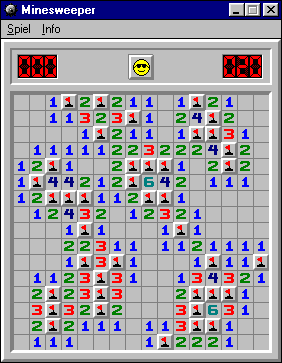
\includegraphics[width=0.9\textwidth]{embeddables/solved_20s_3bv38.png}
        \caption{20s field with a 3BV of 38}
        \label{fig:threebv38}
    \end{subfigure}
    \begin{subfigure}{0.22\textwidth}
        \centering
    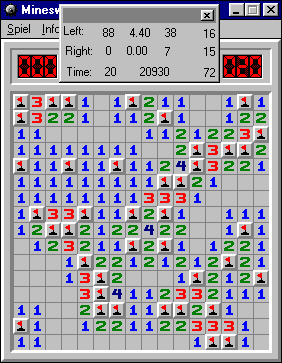
\includegraphics[width=0.9\textwidth]{embeddables/solved_20s_3bv72.png}
        \caption{20s field with a 3BV of 72}
        \label{fig:threebv72}
    \end{subfigure}
    \caption{Fields solvable in 20s with drastically different 3BV scores}
    \label{fig:3BVbad}
\end{figure}


\subsection{Problem Statement - need better than 3bv} \label{awa:minesweeper3BVbad}
So far there exists no metric or combination of metrics that can sufficiently capture the nuances in difficulty of minesweeper boards, and instead players must use a combination of surface-level metrics for a general estimation of difficulty instead.

Considering minesweeper's nature and its difficulty as an NP-hard game, as shown by \citet{kaye2000minesweeper} whose argument we'll explore below, we aim to explore the possibility for a CSP approach to provide a deeper insight into the difficulty of a minesweeper field and allow for more accurate estimation beyond the metrics explored, while also taking into account human factors and investigating how skill correlates to the expected "ideal" difficulty.



\subsection{Logical Complexity of Minesweeper - can use CP algs} \label{awa:minesweeperNPcomplete}
% framing of minesweeper: it's been called a "promise problem" \cite{minesweeperNPmeh}, it's been called a (partially observable) Markov decision problem \cite{msmarkovproblem}
The computational complexity of Minesweeper is well understood to be hard.
\
This fact was first established by a very popular paper by \citet{kaye2000minesweeper},
in which the author simplified minesweeper to what will be referred to as the "minesweeper consistency" problem.
\
This consistency problem is a sub-problem found in minesweeper, that is simpler than playing the whole game but still complex enough to capture the "core" difficulties of minesweeper's computational complexity.
\
\citet{kaye2000minesweeper} defines minesweeper consistency as a problem operating over "a rectangular grid, partially marked with numbers and/or mines, some squares being left blank" which asks whether there exists an assignment of mines to covered cells which is consistent with the numbers revealed in open cells (i.e. all cells numbered $x$ have exactly $x$ neighbouring mines).
\
To prove consistency is an NP-complete problem, \citet{kaye2000minesweeper} begins by establishing that minesweeper is in NP, by showing it is possible to transform a minesweeper field into a boolean satisfiability problem. He states this is done by isolating an arbitrary 3 by 3 grid of cells with a cleared middle cell stating n neighbouring mines, and argues this is equivalent to a boolean satisfiability problem where each clause is a different possible arrangement of mines among the neighbours, with the full 3 by 3 sub-grid being a disjunction of the possible $\begin{pmatrix}8 \\ n\end{pmatrix}$ hidden mine combinations. \citet{kaye2000minesweeper} then assembles these individual SAT problems for 3 by 3 sub-grids into a full statement for the whole board via conjunction.
\
To provide a polynomial time reduction from an NP-complete problem to minesweeper, \citet{kaye2000minesweeper} first shows that it is possible to create boolean logic circuits in minesweeper by showing how to create a simple wire via a mine arrangement where a designated output cell will contain a mine if and only if a designated input cell will contain a mine. \citet{kaye2000minesweeper} then extends this with wire bends and junctions, and finally boolean gates NOT and AND, which provides the basis for the other fundamental logic gates OR and XOR.
\
Using this digital computer, \citet{kaye2000minesweeper} shows how, for any instance of boolean satisfiability, a minesweeper circuit can be constructed where solving for consistency also solves the original SAT instance.
\
Having produced a proof for Minesweeper consistency being NP-complete, \citet{kaye2000minesweeper} then went on to generalise this sub-problem to the whole of Minesweeper, eventually concluding that a typical play through of the game is also NP-complete.

This conclusion is almost as widely accepted as their NP-completeness proof for Minesweeper consistency, but there is some disagreement.
\citet{minesweeperNPmeh} disputes \citet{kaye2000minesweeper}'s generalisation of NP-completeness from consistency to the game as a whole, on the basis that \citet{kaye2000minesweeper} did not consider the possibility that their proposed algorithm for solving general minesweeper via application of the consistency problem is not necessarily the most efficient method.
To explain their objection, \citet{minesweeperNPmeh} introduces a sister sub-problem to Minesweeper consistency - that of Minesweeper inference. This problem takes as input a board similar to consistency, with open cells, closed cells, and flags, and asks whether it is possible to make progress on the given board by identifying a cell as safe or containing a mine, subject to the condition that the board is already consistent and all flags are correct. Intuitively, this asks whether the only remaining actions on the field all force the player to guess, examples for which are shown in \cref{fig:inferenceExample}.
\citet{minesweeperNPmeh} demonstrates that the inference problem is in fact a co-NP problem, and subsequently presents a reduction from the unsatisfiability problem (the co-NP-complete variant of SAT) to Minesweeper inference through a very similar method to \citet{kaye2000minesweeper} - a general reduction for any (un)SAT problem to a computational circuit of logic gates, constructed through the rules of Minesweeper, that solves the respective problem when consistency is solved on the reduced minesweeper problem.

\begin{figure}[htbp]
    \begin{subfigure}{0.21\textwidth}
        \centering
        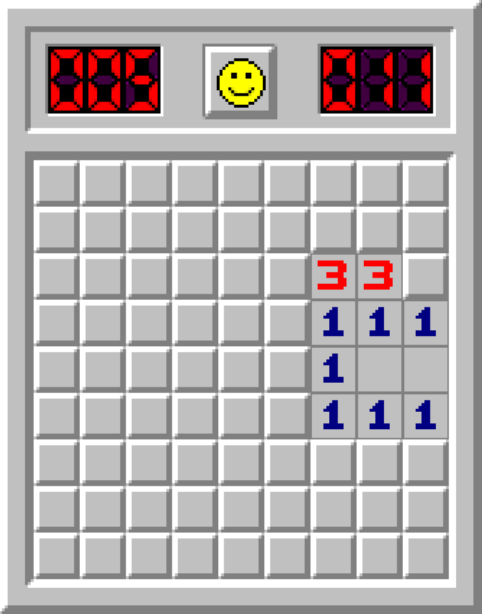
\includegraphics[width=\textwidth]{embeddables/progressableBoardV2.png}
        \caption{Field progressable\\without guessing}
        \label{fig:noGuess}
    \end{subfigure}
    \begin{subfigure}{0.21\textwidth}
        \centering
        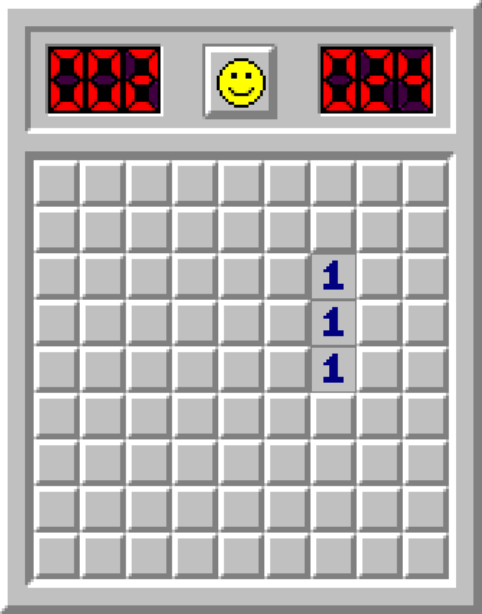
\includegraphics[width=\textwidth]{embeddables/unprogressableBoardV2.png}
        \caption{Field progressable only with guessing}
        \label{fig:guessOnly}
    \end{subfigure}
    \caption{partially solved fields that are progressable with and without guessing}
    \label{fig:inferenceExample}
\end{figure}

% \begin{figure}[htbp]
%     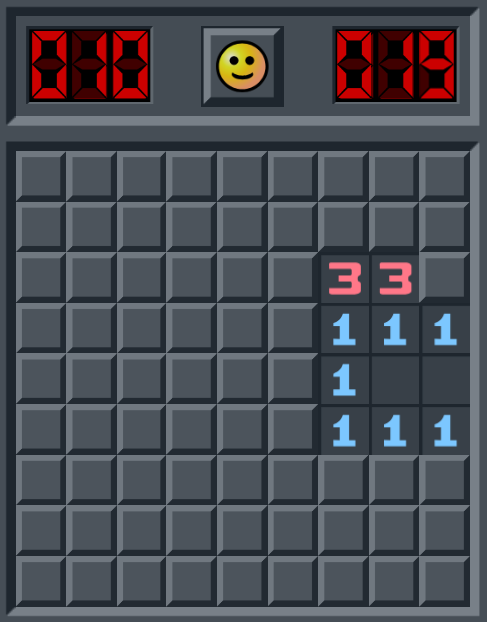
\includegraphics[width=0.20\textwidth]{embeddables/progressableBoard.png}
%     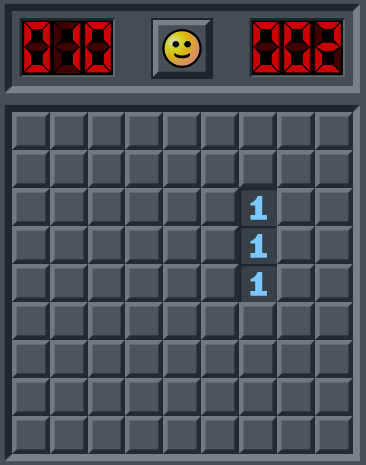
\includegraphics[width=0.20\textwidth]{embeddables/unprogressableBoard.png}
%     \caption{partially solved fields that are progress-able without guessing (left) and not (right)}
%     \label{fig:inferenceExample}
% \end{figure}

\subsubsection{Consistency/Inference Relation} \label{awa:InferenceConsistencyRelation}
\todoPi{this is an (I think) important extension to Inference and Consistency, but it's purely my own design, so I'm not sure I can put it in this section here and take it as fact?} \\
\todoPl{this will be explicitly stated as my own proposal/interpretation on a link between consistency/inference, and should likely be moved into the design somewhere}
\todo{re-write for better explanation}
\todoLg{In the context of a full minesweeper instance, these sub-problems do not suffice to make up the whole solving sequence. A full solve can be broken down into a repeated application of inference, where progress made on an individual instance of inference implicitly keeps the field "consistent".
\
Inference itself can also be defined in terms of consistency.
Inference can only be solvable when Consistency is solvable.
Inference on a field is possible when any cell on that field is solvable, without ambiguity.
This means that, in all possible solutions to Consistency, that same cell takes the same value all the time.
In the special case where there is only one solution to consistency, then Inference is possible on every cell, since no cell is ambiguous.
On the other hand, Inference on a field is not possible if every undecided cell has multiple possible options across all consistency solutions, i.e. there is always ambiguity.
\\
In other words, Inference asks whether the number of unambiguous cells across all Consistency solutions is greater than 0. If there are multiple unambiguous cells, then there are multiple Inference solutions.
\
While the computational complexity of a full minesweeper solve hasn't been explored, the individual steps still comprise NP-hard problems so our research into difficulty will need to focus on inference and develop methods to aggregate difficulty over the repeated occurrences that comprise the full solve of a minesweeper field.}
\\
% \todoOr{consistency but no inference means a forced guess.}
% \todoLi{ multiple consistency means multiple solutions. inference for a cell is only possible where all possible consistency solutions overlap for that cell.
% \\ \\
% no inference and multiple consistency means a forced guess \\
% one consistency solution means inference \\
% any inference and no consistency means there's been a mistake \\
% no inference and no consistency also means there's been a mistake }

% \todoPi{rewrite bellow til pink}
\subsection{Difficulty Manipulation via CSP Strategy Manipulation (MEH; rewrite, dont copy.)} \label{awa:difficultyManipulationAttempts}
\todoPi{this is begging to look into pathfinding, specifically manipulating the pathfinding options that arise whenever the player uses some heuristics or logic}
Knowing minesweeper can be classified as a constraint satisfaction problem, we can look to other studies investigating the difficulty of Constraint Satisfaction Puzzles, for insights that might extend to Minesweeper.
\
Specifically, we look at research in sourcing minesweeper heuristics, applying them, and lastly trying to manipulate them, in order to demonstrate the link between community-learned heuristics (patterns), and the perceived difficulty in the CSP game.

\subsubsection{sourcing common game strategies} \label{awa:playerStudiedTechniquesAreProbabllyMostOfThem}
\todoPi{player skill - says that a small subsection of techniques is already pretty sufficient} 
Before we can look at CSP strategies and how they relate to difficulty, we first need a way to identify strategies in the first place for investigation.
% \todo{place this somewhere with flow}
In \citeauthor{sudokuComputationalModel}'s research on encoding sudoku techniques into a computational model, they rely solely on techniques learned and documented by players through gameplay (specifically - techniques documented in popular puzzle solving books). While such a source may be non-exhaustive, it serves as a good starting point and likely includes most of the frequently encountered techniques.

% which may not seem academically sound, but other authors do the same suggesting community made materials are generally assumed safe by academia and appropriate to base findings on.

\subsubsection{research applying community-researched game strategies} \label{awa:basicHHuristicsIntoAlgorithms}
\todoPi{logical complexity - leading into heuristics that implement RAC}
In Minesweeper, there have been attempts to implement both classical (i.e. intuition or heuristics based) algorithms and constraint-based models, with some of these attempts basing themselves on previously identified human strategies and behaviours.

One such "classical" attempt is the "Single Point" strategy. the concept behind the single point strategy (SP) itself centres around the most common and simplest inferences or patterns that minesweeper players first learn, such as the one shown in \cref{fig:cornerexample}. The technique was formalised into the "single-point" strategy by \citeauthor{minesweeperSinglePoint}. Execution of SP starts by establishing an internal set of known valid moves, which the player picks moves from and executes. upon execution of a move, the set is refreshed with newly identified safe moves. Safe move identification is based on the simplest minesweeper technique - the identification of cases where the number in a cell is exactly equal to the number of neighbouring flagged cells which allows all neighbouring closed cells to be revealed, and secondly the identification of cases where the number of unopened neighbours is equal to the count of a cell, allowing the player to conclude that all neighbouring cells contain mines.

\citeauthor{minesweeperSolverShowdown} outlines a problem with the SP strategy where squares that did not immediately yield useful information are discarded prematurely. To mitigate this, they introduce a "Double Set Single Point" strategy. This strategy is defined as an extension to the simpler single point algorithm. Where SP would discard a square on a minesweeper field that does not fall into either of the 2 conditions for "progress", DSSP instead adds that square to a secondary set Q, that the algorithm returns to once it has exhausted all first-order squares with immediately accessible information for progress.

% \todo{argue the following: single point is just global arc consistency. DSSP is just global arc consistency, but with the memory to turn it into 2-RC, i.e. the next level in k-consistency.}

% \subsubsection{creating levels by manipulating "strategies"} \hfill \\
\subsubsection{research manipulating community-researched game strategies} \label{awa:minimisingSudokuValue}
\todoPi{remove? this is about storytelling in a linear game. minesweeper is non-linear with no story.}
\todoPi{besides the note on the line above, this section generally I think is pretty important in establishing pathfinding. I think it is the main chunk, taking a paper example and then explaining how it turns into the model. problem: it's a paper analysis intertwined with model definition. idk how to lead the fact that the paper reveals the concept of pathfinding, while not actually introducing it.}

In general game design, \citeauthor{marioEndless} focuses on combining mini levels together to form cohesive larger levels and create a "storyline" in a mario level. This is done by applying "Tension Arcs" which organises the order in which sub-levels are combined to maintain a smooth ramp-up in difficulty to a peak in the middle of the level which then starts to decay as the level finishes (effectively, the "story").

This notion of "difficulty regions" is also important in CSP games, for example in \citeauthor{sudokuGenerateBalancedHardness}'s research where they use the concept to get around scaling sudoku boards beyond sizes of 5 blocks (a block being a 3 by 3 sub-section), where the difficulty of solving increases drastically.

% This notion of "difficulty regions" is also present in other CSP games, for example \citeauthor{sudokuGenerateBalancedHardness} who addresses a challenge in generating sudoku boards where the "sub-block" construction of sudoku boards leads to significant jumps in difficulty as board block count increases, most notably at the boundary between 5 and 6 blocks.

To progress difficulty further while not having to scale the board size, they research board generation methods which "hide" complex combinations of constraints in generated fields to control the flow of difficulty.
\
Their approach starts with a given, complete, sudoku field, and creates permutations via specific permissible actions that rearrange the board in fashions which do not violate the rules.
\
They apply difficulty controls as rulesets for this generator,
with the core of their difficulty control being the "balance" of empty cells through rows, columns, and blocks.
\
Their difficulty balancing uses a network representation of sudoku boards, in which there is $n+m$ nodes for each $n$ rows and $m$ columns with nodes being connected if and only if that (row, column) position on the board contains an empty cell. Using this framing, they constrain their generator to enforce a regular bipartite graph, which effectively "balances" empty cells between rows and columns so there does not exist any disproportionately weighted node. Maintaining a node balance then ensures that empty squares are spread out and interact with each other minimally, so the user is only able to make slow consistent progress rather than solving a single empty square for a significant chunk of the board.

This balancing approach via a regular bipartite graph addresses the easiest method for progress in sudoku - filling out empty cells that are alone in an otherwise filled out row/column/block.
Sudoku, much like minesweeper and other logic games, has more complex techniques available to a player beyond the techniques mitigated by these surface-level balancing operations. While the demonstrated difficulty balancing only balances the usability of easier techniques, it brings up an important idea of "technique reward", whose average value and variance could impact the reward in a given map for luck or a gambling-focused play style.

\subsubsection{finding typical path difficulty, with heuristics, to categorise fields} \label{awa:fieldQuantisingWithHeuristics}
% \todoPi{this is kinda an attempt to simulate the skill factor, by using virtual agents with increasingly complex skill (instead of humans). this is also important for our future work in pathfinding, because we propose using this as a substitute for human playthroughs.}
\todoPi{this is broadly a pathfinding section. our future work would ultimately be full path enumeration, but this work is a stepping stone where it considers a small set of paths according to \textit{machines} of different skill. it's a further step than what I do, which is a small set of paths according to \textit{humans} of different skill} 
Getting closer to Minesweeper, \citet{minesweeperGeneration} creates a Minesweeper board generator, and much like \citet{sudokuComputationalModel} they also source field candidates via random placements. In their case however, presumably since Minesweeper boards are much more relaxed in their rules for "consistency", \citeauthor{minesweeperGeneration} does not need to use a complex board generator or permutation scheme. Instead, their approach constructs a board by randomly placing mines in an empty grid and using minesweeper solver algorithms to validate that inference is possible, proposing that this should guarantee the whole field is solvable.
% By the nature of \citeauthor{minesweeperGeneration}'s selected algorithms for inference checking, this generator might arrive at false negatives on some particularly complex generations, since the chosen solvers are not computationally perfect solvers and rather are primarily composed of good-enough polynomial solvers.
\citeauthor{minesweeperGeneration}'s chosen algorithms for inference validation starts with single point, secondly moves on to a backtracking algorithm with complex guessing, thirdly tries a "linear equation solver" which is self-described as an extension to single point, fourthly applies a good-enough polynomial time solver, and lastly tries an algorithm with exponential complexity. All of these algorithms, while increasingly complex, do not exhaustively solve all minesweeper instances and thus opens the generator to the possibility of false negatives on some particularly complex generations.
\todo{$\uparrow$ expand on the algorithms and why they're relevant}

This generator, with a wide selection of different solving options with increasing complexity, was found to be effective in selecting fields with specific "ranks" (the largest number of variables ever needed to consider in a single step in the whole field solve), ranging up to rank 9.

This validation method using increasingly complex solvers is effective at categorising fields according to worst-case difficulty, but doesn't reveal much difficulty information on individual moves beyond revealing the hardest move rank in a solve.





\subsection{Applicable Strategies Can Be Found by Relational Arc Consistency} \label{awa:racIdentifiesTechniques}
\todoPi{this section relates to both logic and skill. specifically, an implementation detail rather than any contribution to the model}
The approaches explored so far, which aim to understand and control difficulty,
demonstrate the important idea of "local difficulty" or "strategy biases" within their given problem.
That is, local portions of a problem instance that necessitate "harder" techniques to solve.

We might then want to look at similar strategy biases within minesweeper fields, to get a more granular understanding of how difficulty is affected.
A method for doing this is already partially demonstrated by \citet{minesweeperNConsistencyAssist}, who aims to create a tool, via constraint programming, to assist players in solving minesweeper fields.
To do this, they give the player the option to ask the computer to apply varying levels of the relational arc consistency algorithm, as defined by \citet{ConstraintProcessingBook}, for three different levels {1,2,3}-RC, and either solve all moves revealed by the algorithm or simply identify them.

Their use of Relational Arc Consistency inadvertently demonstrates how it can relate to minesweeper strategies of varying difficulty, as can be seen in \cref{fig:msRAC}. While their paper does not thoroughly study this relation, their demonstration still supports the idea and provides a good starting point in investigating how constraint satisfaction techniques relate to game solving heuristics learned by humans.

\begin{figure}[htbp]
    \centering
    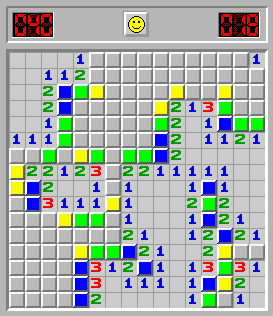
\includegraphics[width=0.5\linewidth]{embeddables/minesweeperTechniques.png}
    \caption{minesweeper field annotated with blue, green, and yellow illustrating possible progress discernable via 1, 2, and 3-RC respectively.}
    \label{fig:msRAC}
\end{figure}

\subsubsection{Relational Arc Consistency} \label{awa:relationalArcConsistencyDiscussionMAYBE}
\todo{insert rundown of RAC}